\section{Imitation Dynamics}
The second evolutionary dynamic to be presented is that of \textit{Imitation Dynamics}. In this case, the new distribution of the population is not calculated strictly as a function of the fitness of each strategy for each generation. Instead, a simpler and perhaps more realistic logic is adopted: in each generation, we identify the strategy (or, in case of a tie, the strategies) that performed best. Then, given a defined number \( K \) of players who change strategy per generation, \( K \) non-optimal strategy players are randomly selected and each adopts one of the optimal strategies, again randomly, in the case of ties.

It is important to highlight that the selection is only made among players who are not already using an optimal strategy, and not among all players in the population. We consider this to reflect reality more accurately --- if a player is already following an optimal strategy, why would they consider changing? This choice has some consequences on the results that are presented below.

To determine the optimal strategy, a score calculation similar to that used in the fitness dynamics case is employed, in order to save computational time. That is, matches between every player are not actually simulated; instead, scores are calculated based on the payoffs of each strategy against each other strategy and the corresponding population sizes.

As will be shown below during the theoretical presentation of the \texttt{TourTheImi} function, this process can be formulated using a Markov chain, where the states are the various possible population distributions, based on the sum of the initial populations (the total population) and the number of strategies involved in the process. The theoretical background is crucial to understand the following implementations: initially, we consider the \( r \)-state Markov chain, where each state represents the individual strategy of each player. For example, for \( N = 5 \) players and 3 strategies, a possible \( r \)-state is (11323). We then consider the \( s \)-states, where a state represents the population of each strategy; in the previous example, the \( s \)-state would be (212). Essentially, this involves grouping various \( r \)-states into one \( s \)-state, which, since we are not truly interested in each individual player but in the total population per strategy, is equivalent. It is shown that the process \( r(t) \) is lumpable and therefore that \( s(t) \) is a Markov chain. This theoretical knowledge is necessary for the implementation of \texttt{TourTheImi} below.

\subsection{The function TourSimImi}
The function that simulates the evolutionary tournament with imitation dynamics is implemented as
\[
[\text{POP}, \text{BST}] = \text{TourSimImi}(B, \text{Strategies}, \text{POP}_0, K, T, J, \text{mode}).
\]
The inputs and outputs of the function are similar to those of \texttt{TourSimFit}, with the additional argument \( K \), an integer value that specifies the number of players who change strategy per generation. The additional argument \texttt{mode} (the function runs with default value \texttt{"Individual"}) can take the values \texttt{"Individual"} and \texttt{"Total"}, and refers to the way in which the optimal strategy is selected: in the \texttt{"Individual"} case, the strategy of the best individual player is returned, while in the \texttt{"Total"} case, the strategy with the highest total score among the players using it is selected. The choice of mode yields significantly different results, as will be shown below.

\subsection{The function TourTheImi}
The \texttt{TourTheImi} function has the form
\[
P = \text{TourTheImi}(B, \text{Strategies}, \text{POP}_0, K, T, J, \text{mode})
\]
with arguments identical to the function \texttt{TourSimImi}, and output the transition matrix \( P \) of the Markov chain of the s-states. In reality, the initial population is used only to determine the total population size of the tournament (so it could simply be replaced by an argument \( N \)), and the number of generations \( J \) is not used at all.

For this analysis, we consider the s-states of the tournament as the number of players using each strategy. For example, for \( N = 9 \), we may have
\[
s_1 = \begin{bmatrix} 0 & 0 & 9 \end{bmatrix}, \quad s_2 = \begin{bmatrix} 0 & 1 & 8 \end{bmatrix},
\]
and so on. Depending on the \texttt{mode} argument, we expect the transition matrix to take different forms. For example, in \texttt{"Individual"} mode and with strategies \texttt{All\_D}, \texttt{All\_C}, and \texttt{TitForTat}, we expect the state
\[
\begin{bmatrix} 0 & 5 & 4 \end{bmatrix}
\]
to be absorbing, since there are no non-optimal players, and therefore it should have only one transition — to itself — with probability 1. In contrast, in the \texttt{"Total"} mode, this state would not be absorbing, as the \texttt{All\_C} strategy accumulates more total points.

Another function is also created:
\[
\text{AnalyzeMarkovChain}(P, \text{POP}_0, \text{Strategies}, \text{Title}),
\]
which is responsible for generating the state transition diagrams shown below. This function, based on the matrix \( P \) calculated by the \texttt{TourTheImi} function and the initial population \texttt{POP0}, classifies the states into transient, absorbing, and the initial state. It also further distinguishes between reachable and unreachable states based on the initial state. It generates a diagram of each state, where the state type is indicated with color, the population of each strategy is shown, the strategy names are labeled (as given by the \texttt{Strategies} argument), and the corresponding transition probabilities are displayed above each transition. The \texttt{Title} argument is the title of the resulting diagram.

\subsection{Simulations - Examples}
Below are some simulations generated by the functions described above, which are of interest. Each simulation is located in a specific example file in the Examples folder and by running the files properly, the exact results presented below are produced.
\subsubsection{1st Simulation - Example usage of Tour\-The\-Imi, Analyze\-Markov\-Chain and Tour\-Sim\-Imi}
In the first simulation \ref{fig:TourTheImi153}, the Markov chain resulting from the strategies $\begin{bmatrix}All\_D & All\_C & TitForTat\end{bmatrix}$ in the mixture $\begin{bmatrix}1 & 5 & 3\end{bmatrix}$ is presented.

From the resulting diagram, we observe that the possible absorbing states are $\begin{bmatrix}9 & 0 & 0\end{bmatrix}$, which corresponds to the dominance of the $All\_D$ strategy, $\begin{bmatrix}0 & 0 & 9\end{bmatrix}$, corresponding to the dominance of the $TitForTat$ strategy, and $\begin{bmatrix}0 & 1 & 8\end{bmatrix}$, corresponding to the dominance of $TitForTat$ with the survival of $All\_C$. From the transition probabilities, shown on the transition arrows, we observe that the last absorbing state has a significantly lower probability of occurring compared to the other two.

Furthermore, we observe that the states in which only the cooperative strategies exist ($All\_C$ and $TitForTat$), i.e., strategies that never defect first and therefore their players achieve equal scores when playing against each other, transition only to themselves, since there are no players with a lower score than the maximum.


	\begin{figure}[h]
	      \centering
	      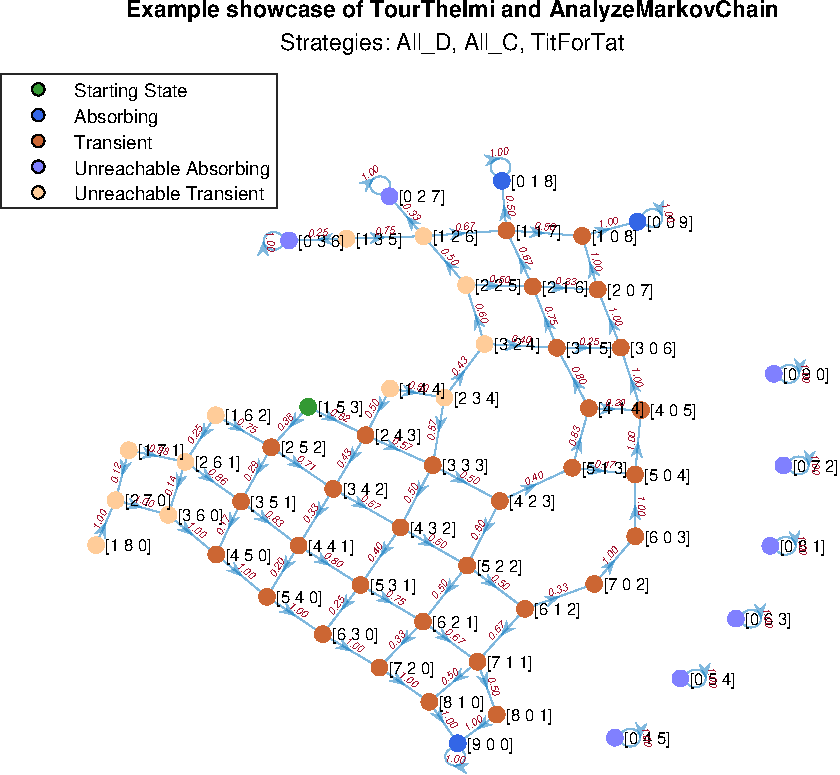
\includegraphics[width=0.95\textwidth]{Example showcase of TourTheImi and AnalyzeMarkovChain.pdf}
	      \caption{Example showcase of TourTheImi and AnalyzeMarkovChain}
	      \label{fig:TourTheImi153}
	\end{figure}
	
In Figure \ref{fig:TourSimImi153}, two executions of the \texttt{TourSimImi} for the strategy mixture of the above simulation are illustrated. We observe that due to the random selection of imitators—i.e., players who do not have the best strategy and switch to one of the better ones—the final mixture of strategies differs for each execution of the program. 

Specifically, in execution (a), we observe 
\[
\begin{bmatrix}1 & 5 & 3\end{bmatrix} \rightarrow^* \begin{bmatrix}9 & 0 & 0\end{bmatrix}
\]
while in execution (b),
\[
\begin{bmatrix}1 & 5 & 3\end{bmatrix} \rightarrow^* \begin{bmatrix}0 & 0 & 9\end{bmatrix},
\]
which, as we analyzed above, are indeed the two most likely absorbing states.

	\begin{figure}[h]
		\centering
		\begin{subfigure}{.5\textwidth}
			\centering
	      	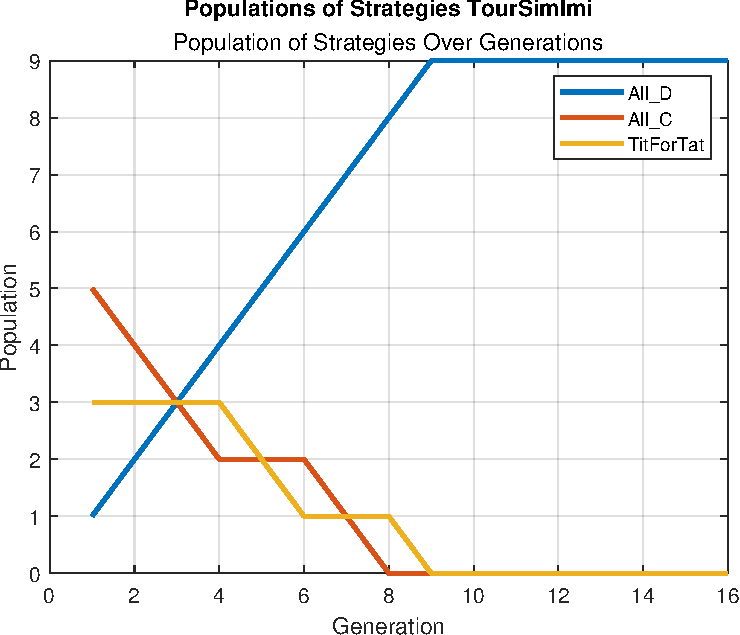
\includegraphics[width=.9\textwidth]{900.pdf}
			\caption{$\begin{bmatrix}9&0&0\end{bmatrix}$}
	      	\label{fig:900}
		\end{subfigure}%
		\begin{subfigure}{.5\textwidth}
			\centering
	      	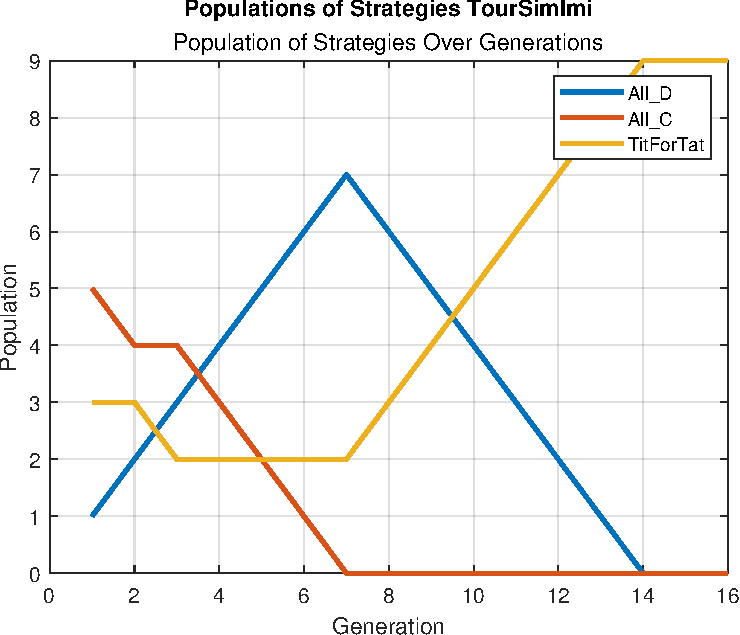
\includegraphics[width=0.90\textwidth]{009.pdf}
			\caption{$\begin{bmatrix}0&0&9\end{bmatrix}$}
	      	\label{fig:009}
		\end{subfigure}
		\caption{Absorbing States may differ even for the same Starting State}
		\label{fig:TourSimImi153}
	\end{figure}

\subsubsection{2nd Simulation - Default mode (Individual) trial for best strategy calculation}
In the next two simulations, an attempt is made to demonstrate the difference in results caused by the different methodologies used to select the best strategy. Initially (Figure \ref{fig:TourTheImiIndividual}), the Markov chain resulting from the initial strategy mixture $\begin{bmatrix}1 & 4 & 5\end{bmatrix}$ and the ``Individual'' selection method is presented, where the best strategy is chosen by comparing the payoffs of the strategies in one-on-one games between each pair of strategies.

The result is similar to that of the first simulation \ref{fig:TourTheImi153}. With some observation, we can envision an imaginary curve connecting the vertices of the states $\begin{bmatrix}8 & 0 & 2\end{bmatrix}, \begin{bmatrix}6 & 1 & 3\end{bmatrix}, \begin{bmatrix}4 & 2 & 4\end{bmatrix}, \begin{bmatrix}2 & 3 & 5\end{bmatrix}$, which separates the basins of attraction of the cooperative and non-cooperative strategies. 

If the system is in a state below this curve, it will end up in the absorbing state where ``All\_D'' dominates. Conversely, if it starts in a state above this curve, it will end up in one of the absorbing states of the cooperative strategies.

	\begin{figure}[h]
	      \centering
	      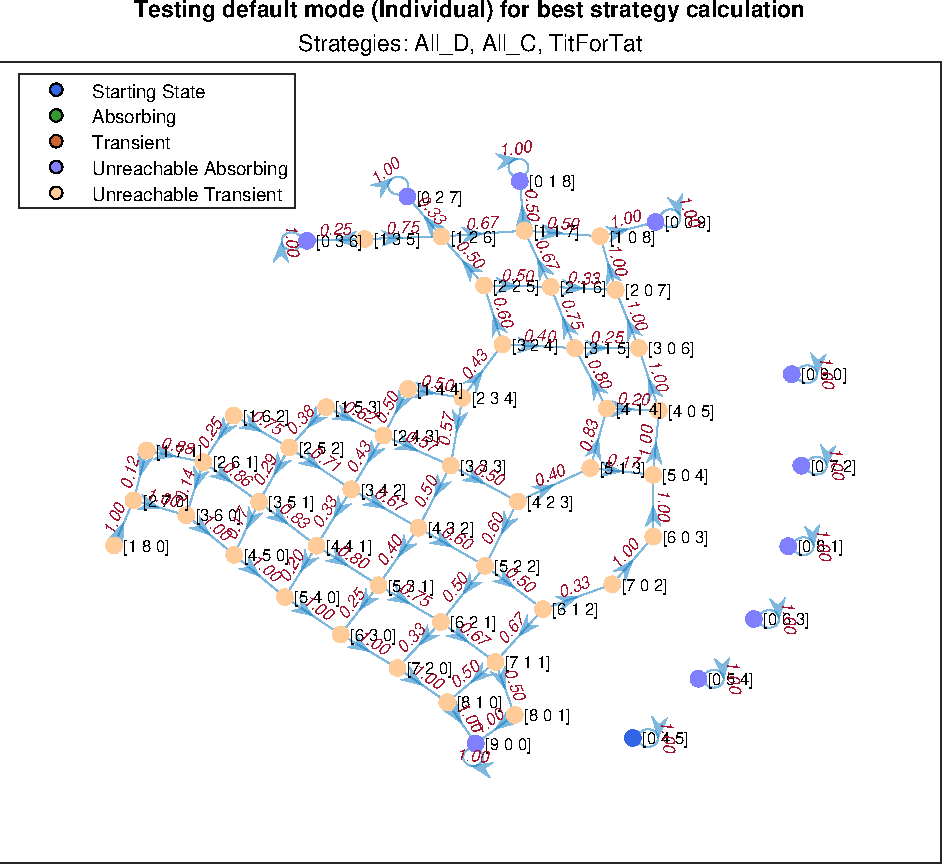
\includegraphics[width=0.95\textwidth]{Testing default mode (Individual) for best strategy calculation.pdf}
	      \caption{Testing default mode (``Individual'') for best strategy calculation with $POP0=\begin{bmatrix}1&4&5\end{bmatrix}$}
	      \label{fig:TourTheImiIndividual}
	\end{figure}
\subsubsection{3rd Simulation - ``Total'' mode trial for best strategy calculation}
In the third simulation (Figure \ref{fig:TourTheImiTotal}), with the same initial strategy mixture $\begin{bmatrix}1 & 4 & 5\end{bmatrix}$ and using the ``Total'' method—i.e., comparing the players' payoffs in each state (as computed by Axelrod) using the populations of the state, and selecting as the best strategy the one belonging to the player with the highest total payoff—we observe different behavior.

In contrast to the previous simulation (Figure \ref{fig:TourTheImiIndividual}), here we observe that the diagram is divided into three distinct subgraphs.

The first subgraph, which includes the initial state, is the only one that contains a reachable absorbing state ($\begin{bmatrix}0 & 0 & 10\end{bmatrix}$), corresponding to the dominance of ``TitForTat''. This occurs because, under the ``Total'' mode for selecting the best strategy, the cooperative strategies collaborate with each other and, due to their greater numbers, overcome the advantage that defection gives to ``All\_D''.

The second subgraph includes the absorbing state where ``All\_D'' dominates ($\begin{bmatrix}10 & 0 & 0\end{bmatrix}$), but this state, as well as all the transitional states in this subgraph, are unreachable for the reason described above.

Finally, the third subgraph includes the absorbing state where ``All\_C'' dominates ($\begin{bmatrix}0 & 10 & 0\end{bmatrix}$), which is also unreachable, as are all the transitional states in this subgraph, for the same reason. 

\subsubsection{4th Simulation - Sensitivity of Imitation Dynamics, mode='Individual', to population's size - Case N=3}
For the next four simulations, the sensitivity of the imitation dynamics in the case of ``Individual'' mode to the total population's size is discussed. For all following simulations, the population consists of members of the following three strategies: \texttt{All\_C}, \texttt{All\_D} and \texttt{Grim} (which in this case is an equivalent strategy to \texttt{TitForTat}). Another important aspect to discuss is the form of the plots produced; a new function PlotStateTransitionGraph is used in order to plot the possible states of the Markov Chain in a triangular form. More specifically, the x-axis of the plot refers to the population of \texttt{All\_D}, the y-axis represents the population of \texttt{Grim} and, since the total population $N$ remains constant, the population of \texttt{All\_C} increases as we move towards the bottom-left of the plot. 

The analysis begins with the simple case of $N=3$. This is the proper instance to comment on the colors of the vertices; the color is produced by calculating the final state probability matrix (by raising the calculated matrix $P$ to a sufficiently large power). The more red a vertex appears, the more likely this population distribution is to lead to the domination of \texttt{All\_D}. The more blue it appears, the more likely it is to lead to the domination of \texttt{Grim}. Lastly, the more green it is, the more likely it is to lead to \texttt{All\_C} domination. You may also notice a few black vertices; these are caused by the fact that for some population distributions (as we also saw earlier) the transition to total dominating states like the ones described above is impossible; with the current dynamics, for example, in a population of only \texttt{All\_C} and \texttt{Grim}, no changes happen to the strategy distribution, meaning the state is also absorbing (if the simulation starts there, it ends there).

We begin to notice a trend in the case $N=3$; only one vertex is green, the vertex where all 3 players follow the \texttt{All\_C} strategy. States in the far left side of the plot are, as discussed earlier, black, except for the one on the top, which is blue (all 3 players follow the \texttt{Grim} strategy). Lastly, there is a distinction between states that lead to \texttt{All\_D} domination and states that lead to \texttt{Grim} domination, with no states possibly leading to both; thus, in the case $N=3$ the winning strategy is deterministic to the initial population. The result can be seen in Figure \ref{fig:Sensitivity of Imitation Dynamics, mode='Individual', to population's size}, subfigure (a). Run example18 of the Examples folder (after reading Quickstart guide) to recreate the figure.

\subsubsection{5th Simulation - Sensitivity of Imitation Dynamics, mode='Individual', to population's size - Case N=5}
In the next simulation, the total population is increased to 5. It is expected that the overall trend will continue, but with the increase in population we at some point expect to see states that may lead to both \texttt{All\_D} domination and states that lead to \texttt{Grim} domination. That is precisely the case; as we can see by the colors of the vertices and by the edges added to the graph, states 9 and 13 both have this property. It should also be noted that state 8 may possibly lead to state 7 as well as the expected state 1, the domination of \texttt{Grim} state. This happens because the non-best strategies of this state are \texttt{All\_D} and \texttt{All\_C}; using $K=1$, as in this example, it is random whether the defector or the cooperator switch strategies first, and thus it is random whether the \texttt{Grim} strategy totally dominates. The result can be seen in Figure \ref{fig:Sensitivity of Imitation Dynamics, mode='Individual', to population's size}, subfigure (b). Run example19 of the Examples folder (after reading Quickstart guide) to recreate the figure.

\subsubsection{6th Simulation - Sensitivity of Imitation Dynamics, mode='Individual', to population's size - Case N=10}
As the population keeps increasing, as in the case of this simulation, where the total population is increased to 10, we expect the results to change as before; more states are going to possibly lead to both \texttt{All\_D} domination and states that lead to \texttt{Grim} domination. Also, the higher and to the right of the plot, the more likely \texttt{Grim} domination is to occur. The expected results are the ones also reproduced in the Figure. The result can be seen in Figure \ref{fig:Sensitivity of Imitation Dynamics, mode='Individual', to population's size}, subfigure (c). Run example20 of the Examples folder (after reading Quickstart guide) to recreate the figure.

\subsubsection{7th Simulation - Sensitivity of Imitation Dynamics, mode='Individual', to population's size - Case N=100}
Lastly, one final large increase to the population to $N=100$ is made, which aims to showcase a more continuous form of the graph; in this case, the exact possible transitions of each state are not visible, however the colors of the vertices ``paint'' (pun intended) a complete picture of the situation. More specifically, it is made clear where the states that lead to each possible final state reside inside the graph. This generalizes the concept presented thus far; a red triangle in the bottom left of states that lead to \texttt{All\_D} domination, a blue triangle in the top right of states that lead to \texttt{Grim} domination, a purple line of states possibly leading to both separating the two, a green vertex in the bottom left representing the \texttt{All\_C} domination (from the start) and a black line in the left representing possible absorbing states different from the ones with a single strategy alive. The result can be seen in Figure \ref{fig:Sensitivity of Imitation Dynamics, mode='Individual', to population's size}, subfigure (d). Run example21 of the Examples folder (after reading Quickstart guide) to recreate the figure.

\subsubsection{8th Simulation - Sensitivity of Imitation Dynamics, mode='Individual', to payoff matrix - Case a=3.2}
For all previous 4 simulations, the payoff matrix was regarded to be constant and equal to $B = \begin{bmatrix} 3 & 1 \\ 4 & 2 \end{bmatrix}$. As discussed during the analysis of the Fitness Dynamics, the payoff matrix can drastically change the results of a simulation. Thus, for the next 4 simulations, the total population is kept constant $N=10$ and the payoff matrix is changed with the forms $B = \begin{bmatrix} a & 1 \\ 4 & 2 \end{bmatrix}$, with $a \in [3,4)$. This means that the payoff of the cooperation-cooperation result will be increased and the results will be observed. It is expected that such an increase will eventually lead to more strategies leading to the domination of the nice strategies (i.e. \texttt{Grim} domination). 

The analysis begins with the case $a = 3.2$. The result, as expected, is similar to the case of $a=3$ which was indirectly presented in the 6th Simulation, with only a few more strategies leading to \texttt{Grim} domination. The result can be seen in Figure \ref{fig:Sensitivity of Imitation Dynamics, mode='Individual', to payoff matrix}, subfigure (a). Run example22 of the Examples folder (after reading Quickstart guide) to recreate the figure.

\subsubsection{9th Simulation - Sensitivity of Imitation Dynamics, mode='Individual', to payoff matrix - Case a=3.4}
The payoff is increased to $a=3.4$, with the overall effect of the increase becoming more visible. The blue triangle in the top right is expanding towards the bottom left, meaning that even in the cases with a lot of initial \texttt{All\_C} members, because the cooperation payoff is increased a lot, it is easier for the \texttt{Grim} strategy to become the most viable. Thus, the general trend is for the blue triangle to approach the bottom left of the plot. The result can be seen in Figure \ref{fig:Sensitivity of Imitation Dynamics, mode='Individual', to payoff matrix}, subfigure (b). Run example23 of the Examples folder (after reading Quickstart guide) to recreate the figure.

\subsubsection{10th Simulation - Sensitivity of Imitation Dynamics, mode='Individual', to payoff matrix - Case a=3.6}
The further increase to $a=3.6$ further increases the blue vertices in the way discussed above. The result can be seen in Figure \ref{fig:Sensitivity of Imitation Dynamics, mode='Individual', to payoff matrix}, subfigure (c). Run example24 of the Examples folder (after reading Quickstart guide) to recreate the figure.

\subsubsection{11th Simulation - Sensitivity of Imitation Dynamics, mode='Individual', to payoff matrix - Case a=3.8}
Lastly, with the increase to $a=3.8$, the blue triangle becomes a right triangle, meaning the only red states are the ones in the complete bottom of the plot, no longer forming a triangle. It should also be noted that there are no more purple states; the result once again becomes deterministic. It should come as no surprise that there still exist red states; the first line represents an initial population of only \texttt{All\_C} and \texttt{All\_D}, clearly making \texttt{All\_D} the better strategy and leading to red coloring. The line above that corresponds to a single \texttt{Grim} participant in the initial population. The single \texttt{Grim} participant can only ever nearly tie with the \texttt{All\_D} members, and each \texttt{All\_D} member still gets more points from facing the \texttt{All\_C} members than the participant of \texttt{Grim} does, thus again making \texttt{All\_D} the best strategy. The result can be seen in Figure \ref{fig:Sensitivity of Imitation Dynamics, mode='Individual', to payoff matrix}, subfigure (d). Run example25 of the Examples folder (after reading Quickstart guide) to recreate the figure.

\subsubsection{12th Simulation - Sensitivity of Imitation Dynamics, mode='Total', to population's size - Case N=3}

\subsubsection{13th Simulation - Sensitivity of Imitation Dynamics, mode='Total', to population's size - Case N=5}

\subsubsection{14th Simulation - Sensitivity of Imitation Dynamics, mode='Total', to population's size - Case N=10}

\subsubsection{15th Simulation - Sensitivity of Imitation Dynamics, mode='Total', to population's size - Case N=100}

\subsubsection{16th Simulation - Sensitivity of Imitation Dynamics, mode='Total', to payoff matrix - Case a=3.2}

\subsubsection{17th Simulation - Sensitivity of Imitation Dynamics, mode='Total', to payoff matrix - Case a=3.4}

\subsubsection{18th Simulation - Sensitivity of Imitation Dynamics, mode='Total', to payoff matrix - Case a=3.6}

\subsubsection{19th Simulation - Sensitivity of Imitation Dynamics, mode='Total', to payoff matrix - Case a=3.8}
	\begin{figure}[h]
	      \centering
	      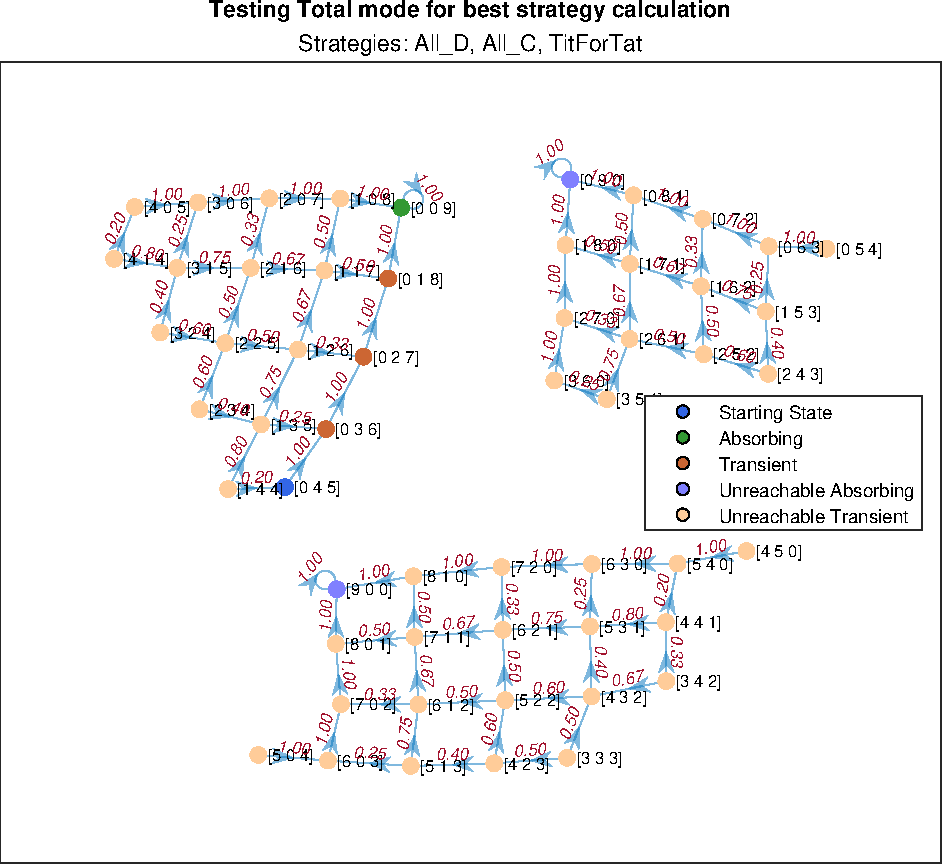
\includegraphics[width=0.95\textwidth]{Testing Total mode for best strategy calculation}
	      \caption{Testing ``Total'' mode for best strategy calculation with $POP0=\begin{bmatrix}1&4&5\end{bmatrix}$}
	      \label{fig:TourTheImiTotal}
	\end{figure}
	
	\begin{figure}[h]
		\centering
		\begin{subfigure}[t]{.49\textwidth}
			\centering
			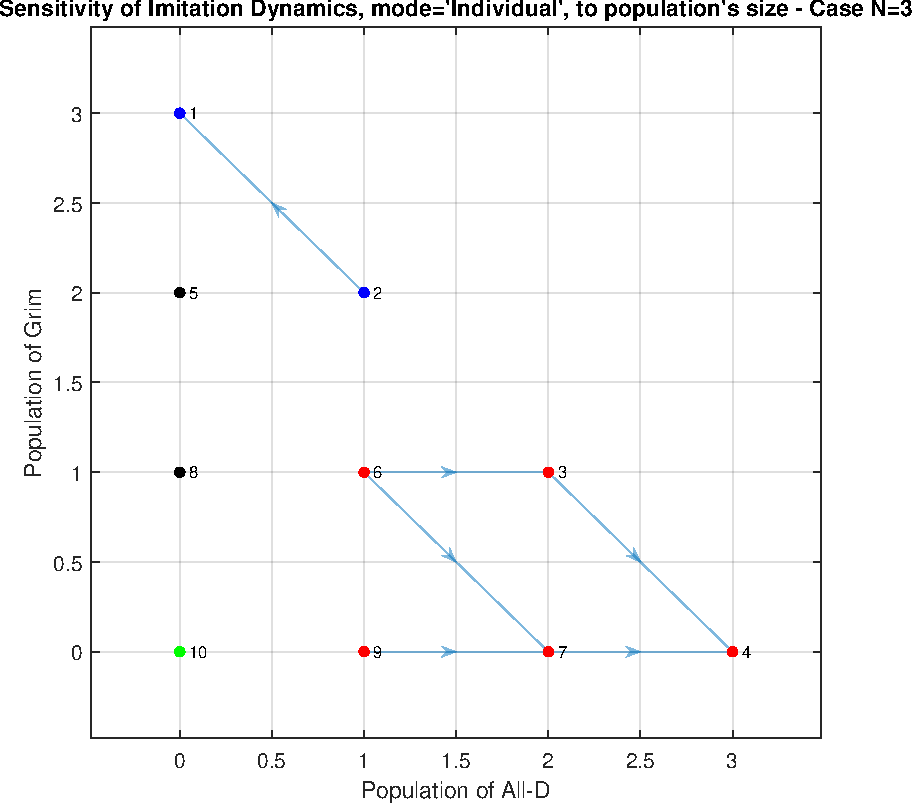
\includegraphics[height=0.8\textwidth]{Sensitivity of Imitation Dynamics, mode='Individual', to population's size - Case N=3}
			\caption{Case $N=3$}
			\label{fig:example18}
		\end{subfigure}
		\begin{subfigure}[t]{.49\textwidth}
			\centering
			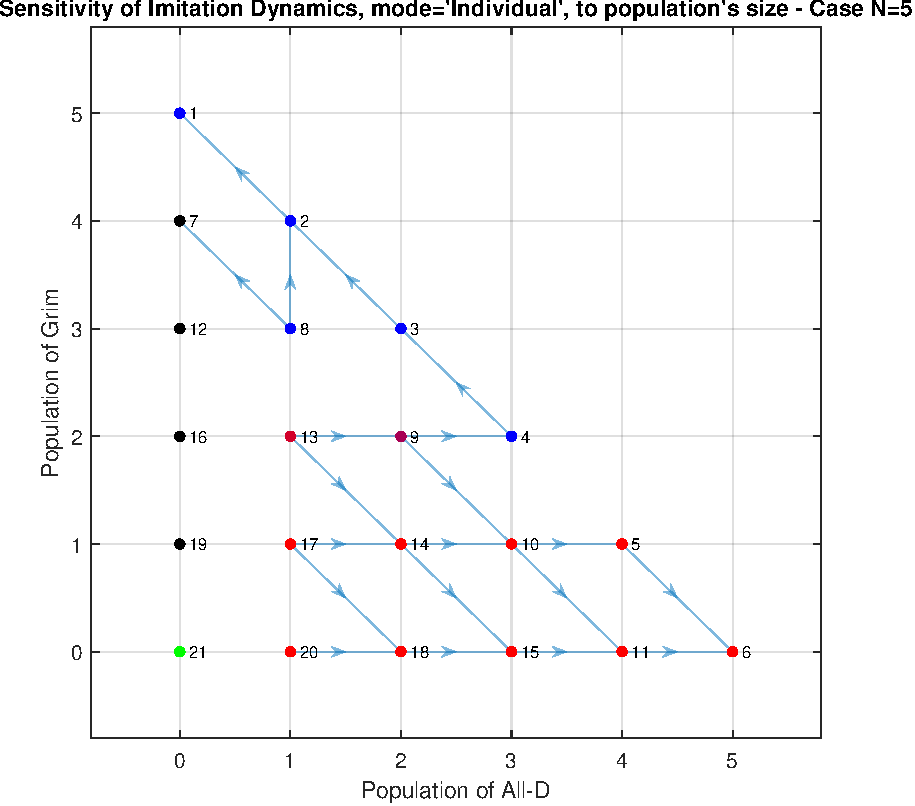
\includegraphics[height=0.8\textwidth]{Sensitivity of Imitation Dynamics, mode='Individual', to population's size - Case N=5}
			\caption{Case $N=5$}
			\label{fig:example19}
		\end{subfigure}
		\par\vspace{1em}
		\begin{subfigure}[t]{.49\textwidth}
			\centering
			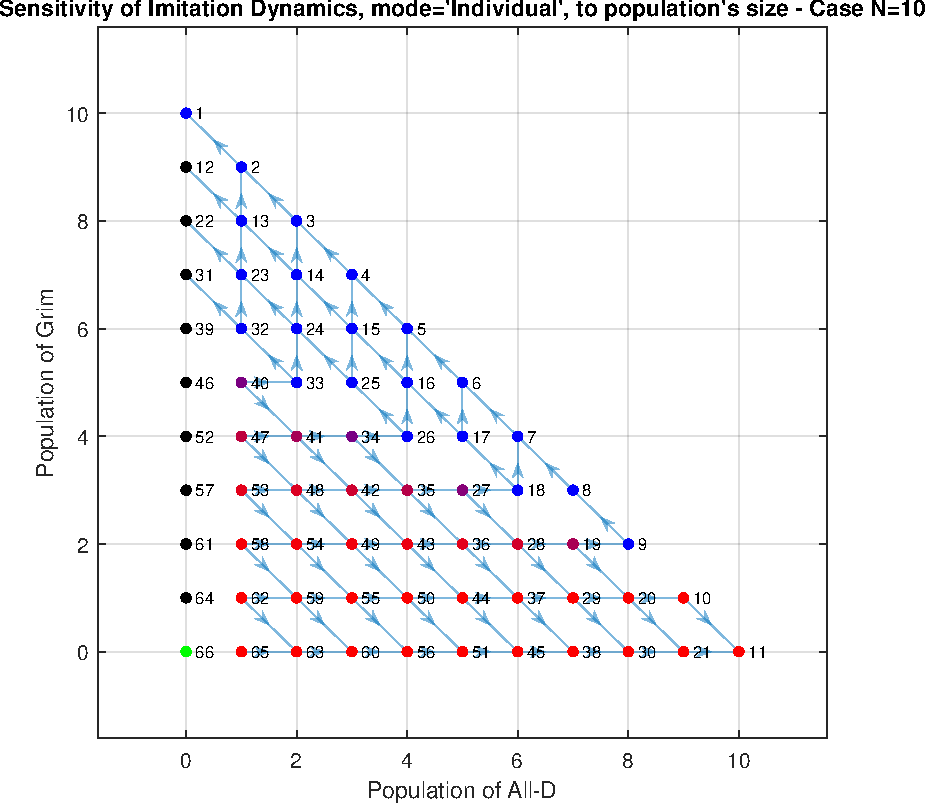
\includegraphics[height=0.8\textwidth]{Sensitivity of Imitation Dynamics, mode='Individual', to population's size - Case N=10}
			\caption{Case $N=10$}
			\label{fig:example20}
		\end{subfigure}
		\begin{subfigure}[t]{.49\textwidth}
			\centering
			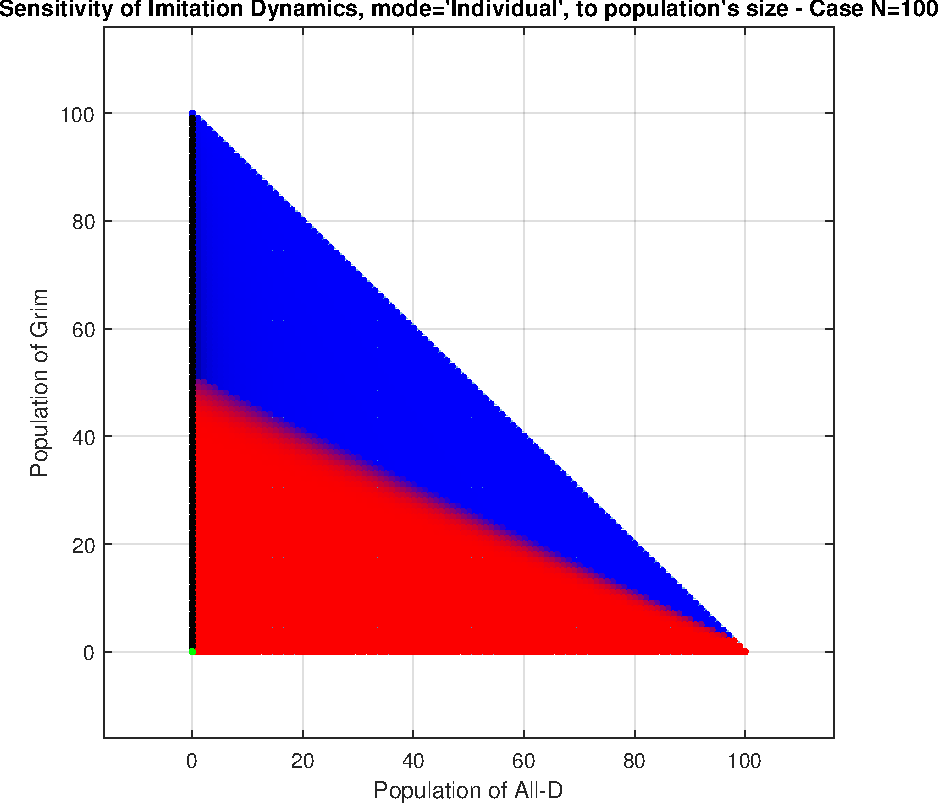
\includegraphics[height=0.8\textwidth]{Sensitivity of Imitation Dynamics, mode='Individual', to population's size - Case N=100}
			\caption{Case $N=100$}
			\label{fig:example21}
		\end{subfigure}
		\caption{Sensitivity of Imitation Dynamics (mode=``Individual'') to population size for $B = \begin{bmatrix} 3 & 1 \\ 4 & 2 \end{bmatrix}$}
		\label{fig:Sensitivity of Imitation Dynamics, mode='Individual', to population's size}
	\end{figure}
	
	\begin{figure}[h]
		\centering
		\begin{subfigure}{.49\textwidth}
			\centering
			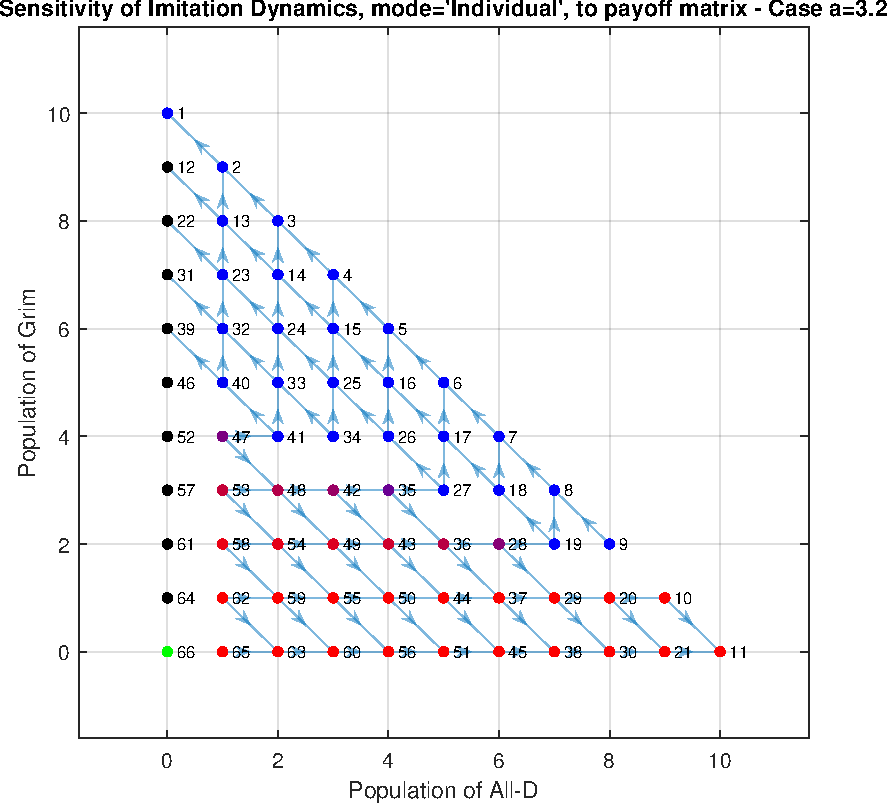
\includegraphics[width=\textwidth]{Sensitivity of Imitation Dynamics, mode='Individual', to payoff matrix - Case a=3.2}
			\caption{Case $a=3.2$}
			\label{fig:example22}
		\end{subfigure}
		\begin{subfigure}{.49\textwidth}
			\centering
			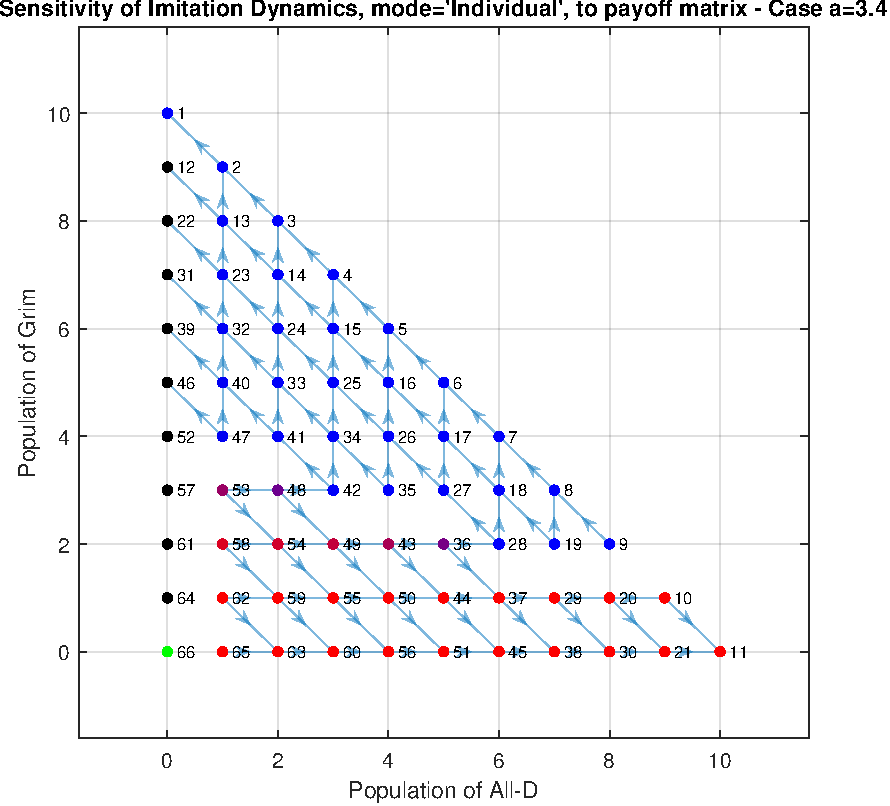
\includegraphics[width=\textwidth]{Sensitivity of Imitation Dynamics, mode='Individual', to payoff matrix - Case a=3.4}
			\caption{Case $a=3.4$}
			\label{fig:example23}
		\end{subfigure}
		\vspace{0.5em}
		\begin{subfigure}{.49\textwidth}
			\centering
			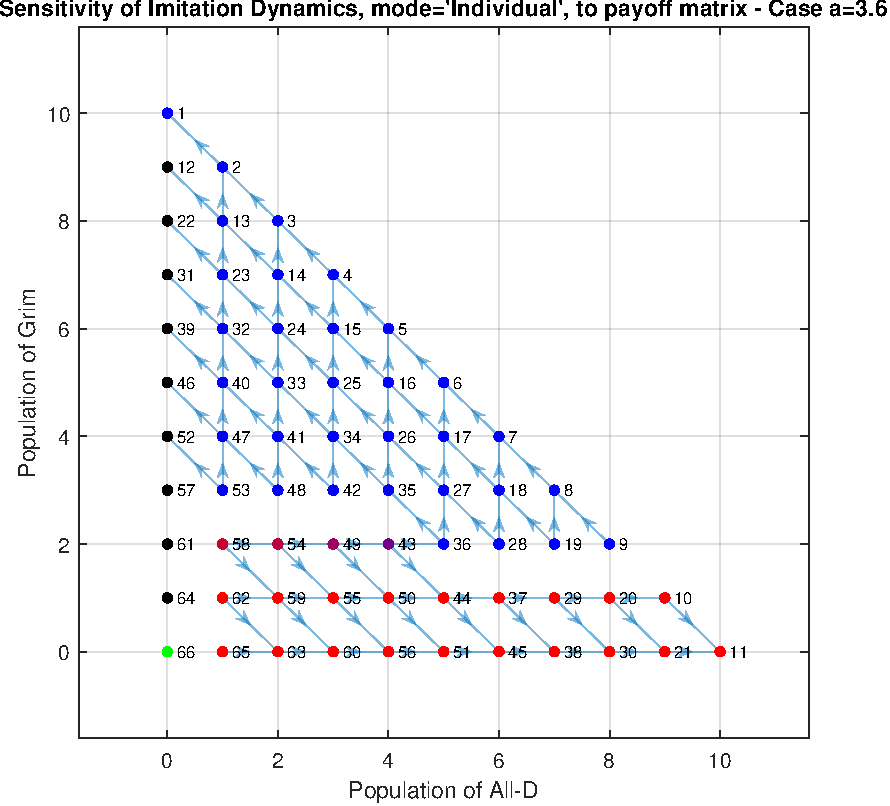
\includegraphics[width=\textwidth]{Sensitivity of Imitation Dynamics, mode='Individual', to payoff matrix - Case a=3.6}
			\caption{Case $a=3.6$}
			\label{fig:example24}
		\end{subfigure}
		\begin{subfigure}{.49\textwidth}
			\centering
			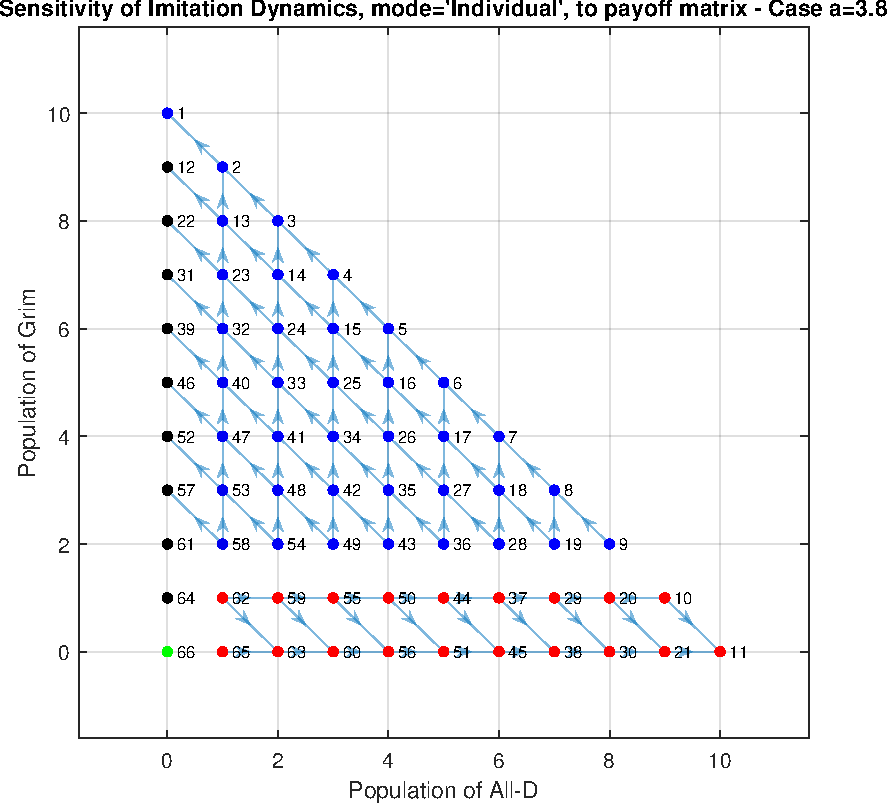
\includegraphics[width=\textwidth]{Sensitivity of Imitation Dynamics, mode='Individual', to payoff matrix - Case a=3.8}
			\caption{Case $a=3.8$}
			\label{fig:example25}
		\end{subfigure}
		\caption{Sensitivity of Imitation Dynamics (mode=``Individual'') to payoff matrix parameter $a$ for $B = \begin{bmatrix} a & 1 \\ 4 & 2 \end{bmatrix}$ and $N=10$}
		\label{fig:Sensitivity of Imitation Dynamics, mode='Individual', to payoff matrix}
	\end{figure}
	
	\begin{figure}[h]
		\centering
		\begin{subfigure}[t]{.49\textwidth}
			\centering
			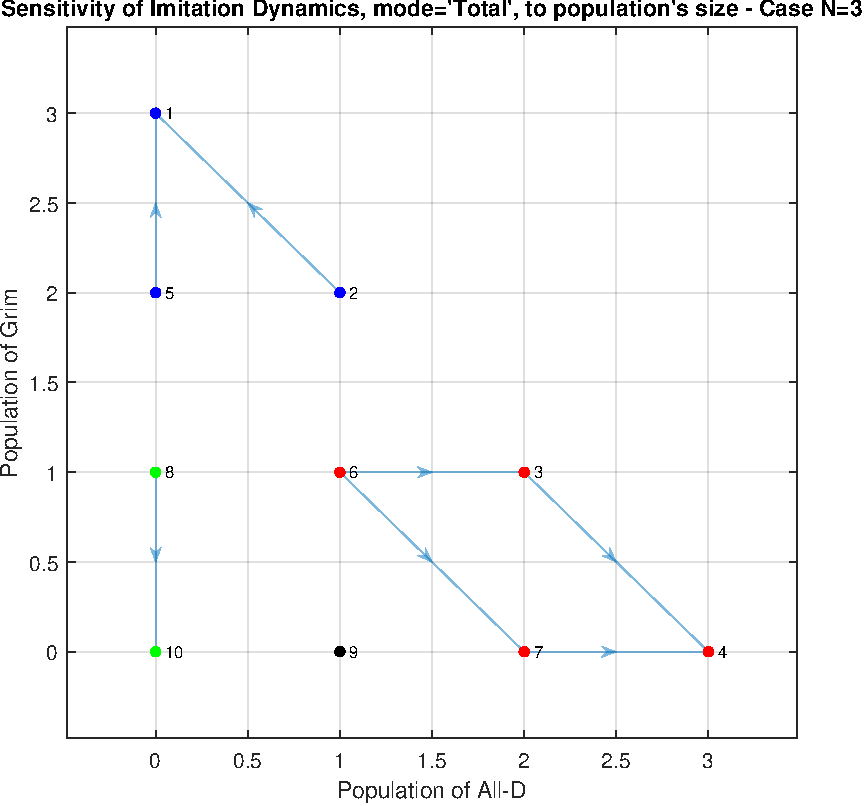
\includegraphics[height=0.9\textwidth]{Sensitivity of Imitation Dynamics, mode='Total', to population's size - Case N=3}
			\caption{Case $N=3$}
			\label{fig:example26}
		\end{subfigure}
		\begin{subfigure}[t]{.49\textwidth}
			\centering
			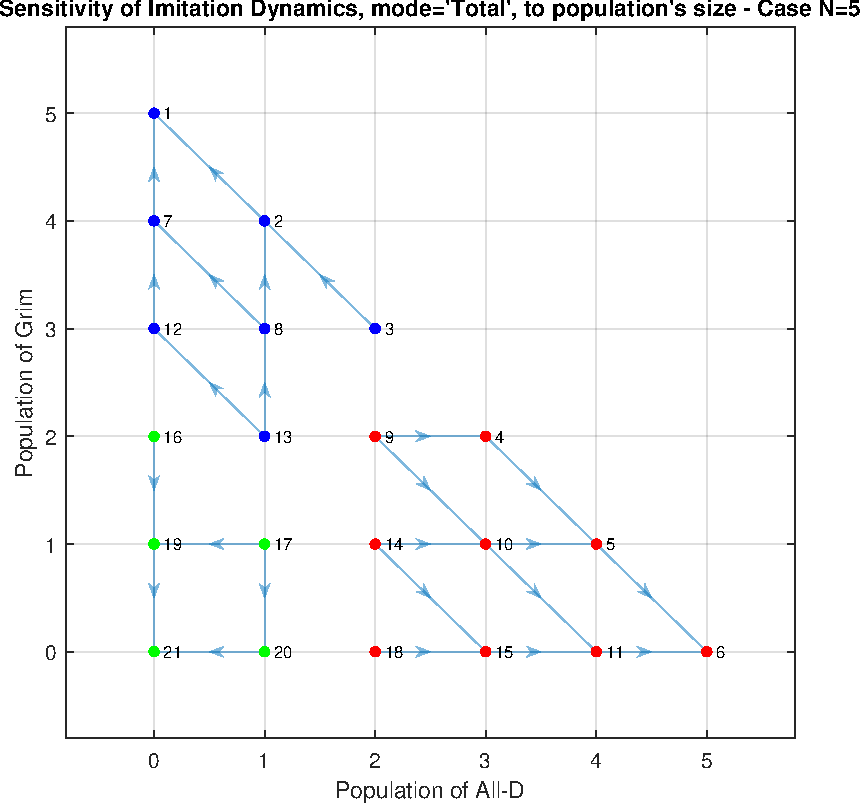
\includegraphics[height=0.9\textwidth]{Sensitivity of Imitation Dynamics, mode='Total', to population's size - Case N=5}
			\caption{Case $N=5$}
			\label{fig:example27}
		\end{subfigure}
		\begin{subfigure}[t]{.49\textwidth}
			\centering
			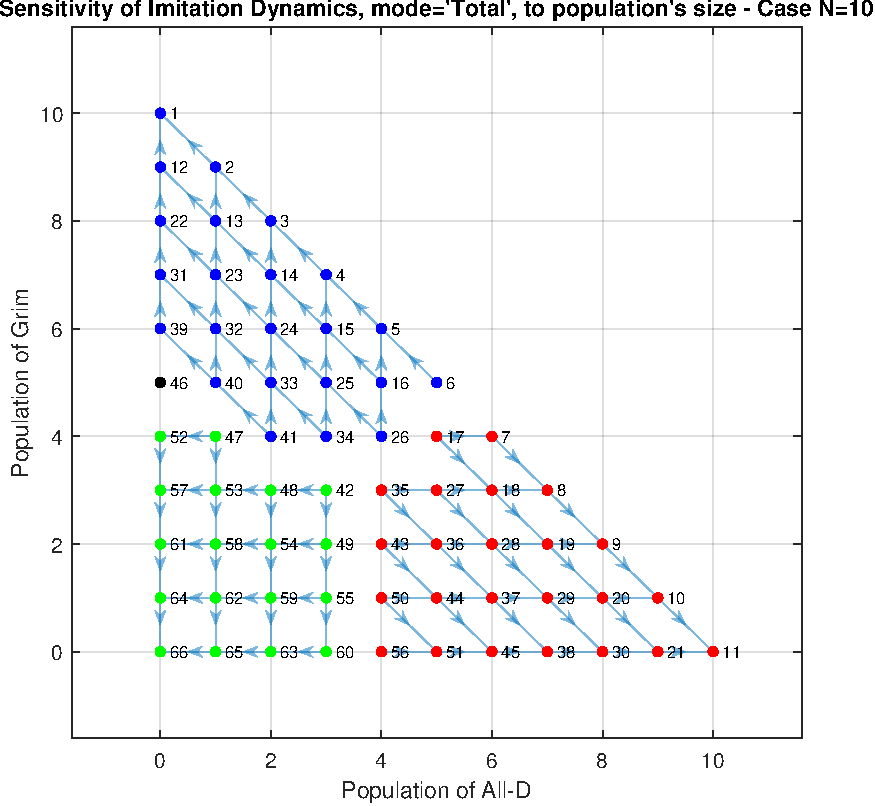
\includegraphics[height=0.9\textwidth]{Sensitivity of Imitation Dynamics, mode='Total', to population's size - Case N=10}
			\caption{Case $N=10$}
			\label{fig:example28}
		\end{subfigure}
		\begin{subfigure}[t]{.49\textwidth}
			\centering
			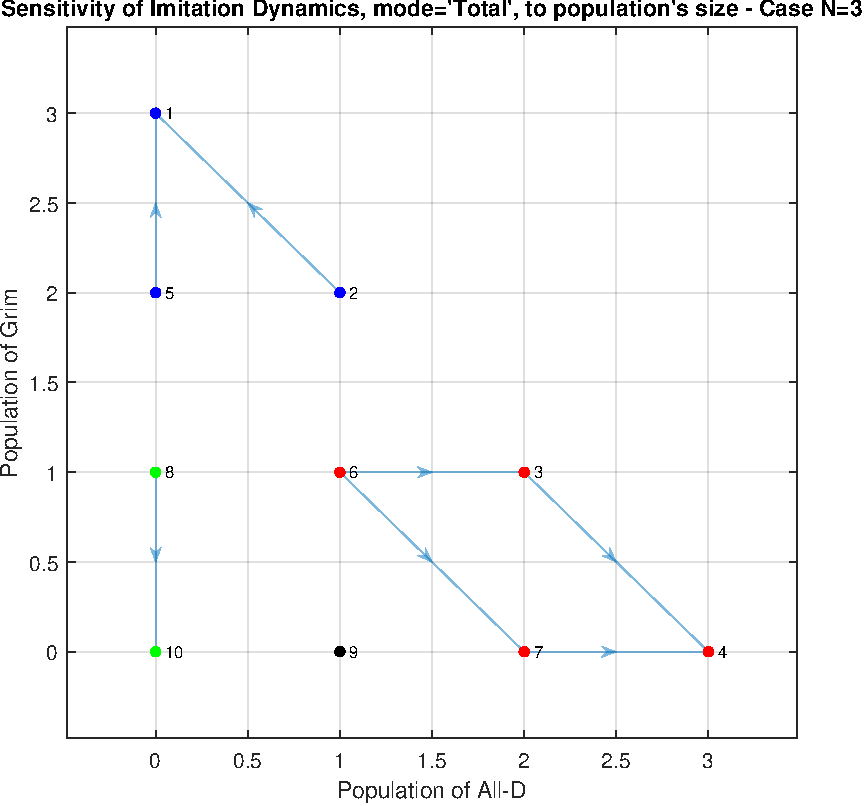
\includegraphics[height=0.9\textwidth]{Sensitivity of Imitation Dynamics, mode='Total', to population's size - Case N=3}
			\caption{Case $N=100$}
			\label{fig:example29}
		\end{subfigure}
		\caption{Sensitivity of Imitation Dynamics (mode=``Total'') to population size for $B = \begin{bmatrix} 3 & 1 \\ 4 & 2 \end{bmatrix}$}
		\label{fig:Sensitivity of Imitation Dynamics, mode='Total', to population's size}
	\end{figure}
	
	\begin{figure}[h]
		\centering
		\begin{subfigure}{.49\textwidth}
			\centering
			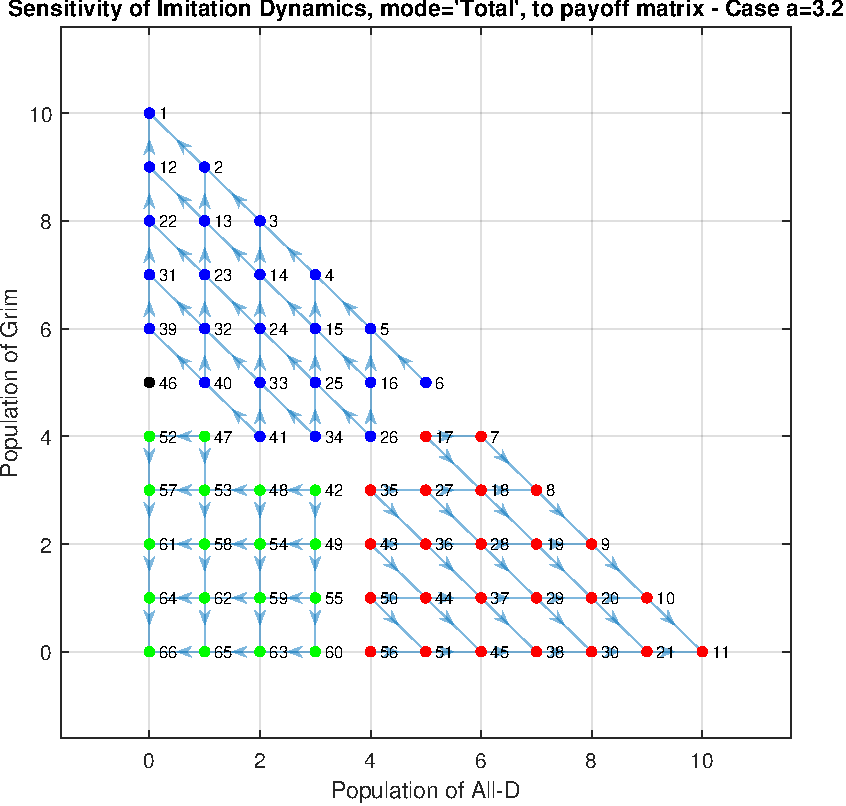
\includegraphics[height=0.9\textwidth]{Sensitivity of Imitation Dynamics, mode='Total', to payoff matrix - Case a=3.2}
			\caption{Case $a=3.2$}
			\label{fig:example30}
		\end{subfigure}
		\begin{subfigure}{.49\textwidth}
			\centering
			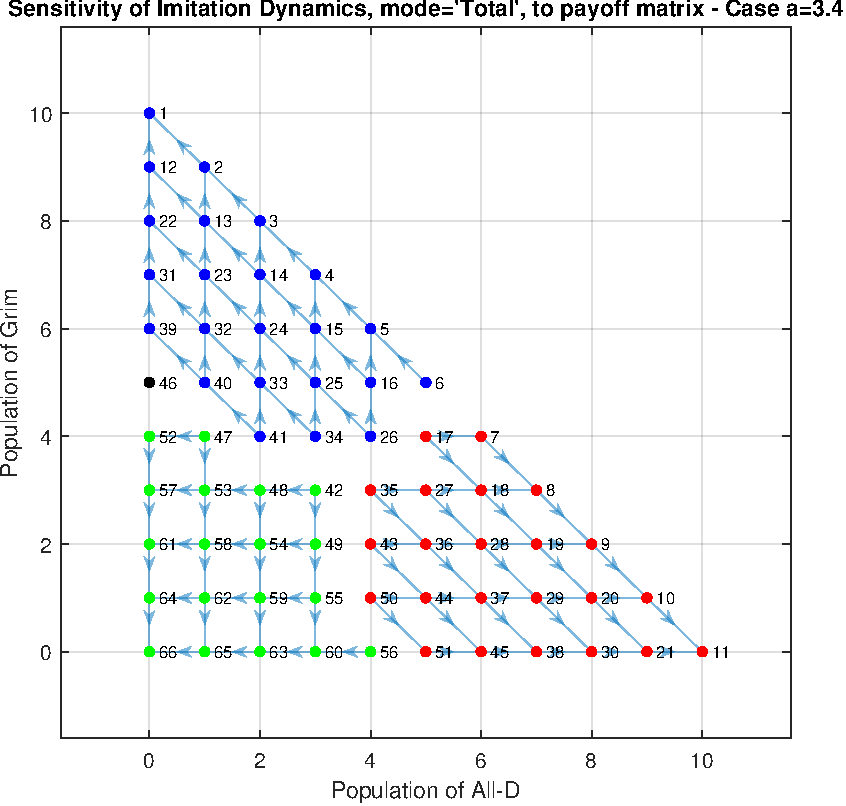
\includegraphics[height=0.9\textwidth]{Sensitivity of Imitation Dynamics, mode='Total', to payoff matrix - Case a=3.4}
			\caption{Case $a=3.4$}
			\label{fig:example31}
		\end{subfigure}
		\vspace{0.5em}
		\begin{subfigure}{.49\textwidth}
			\centering
			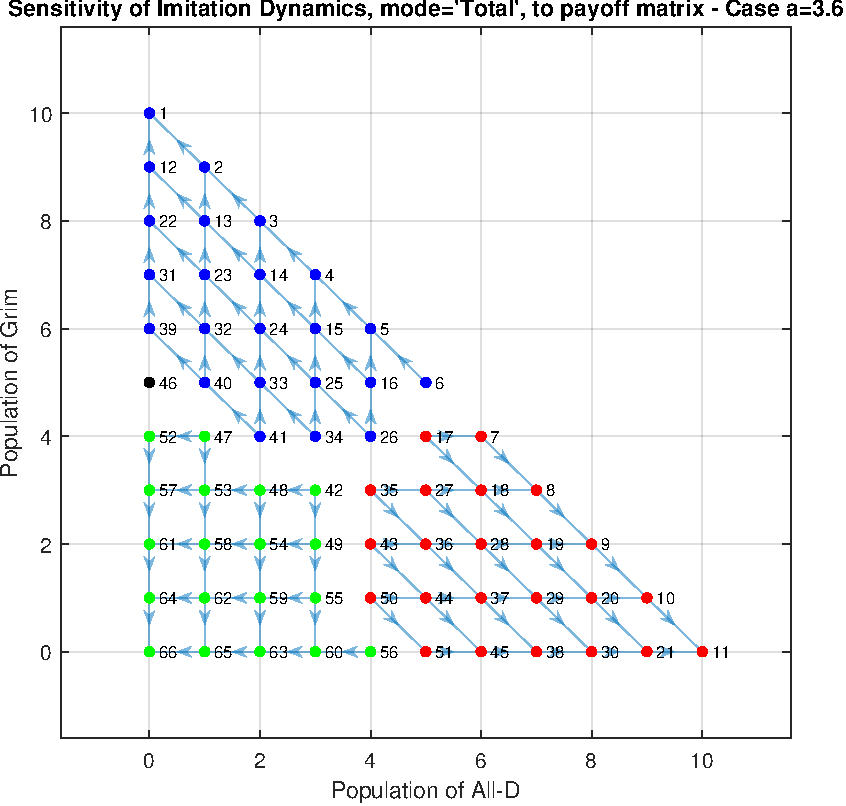
\includegraphics[height=0.9\textwidth]{Sensitivity of Imitation Dynamics, mode='Total', to payoff matrix - Case a=3.6}
			\caption{Case $a=3.6$}
			\label{fig:example32}
		\end{subfigure}
		\begin{subfigure}{.49\textwidth}
			\centering
			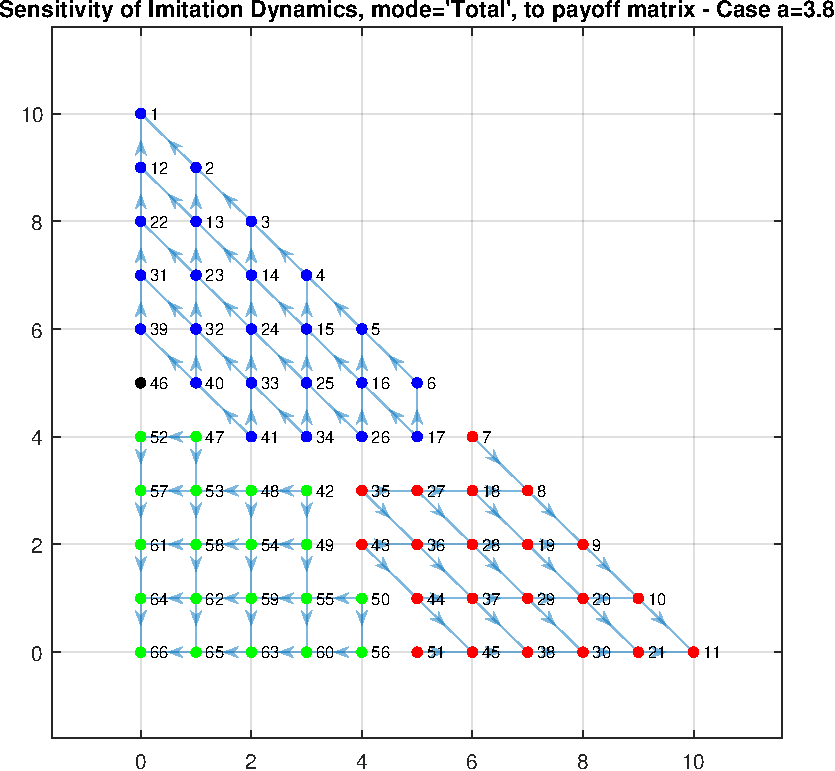
\includegraphics[height=0.9\textwidth]{Sensitivity of Imitation Dynamics, mode='Total', to payoff matrix - Case a=3.8}
			\caption{Case $a=3.8$}
			\label{fig:example33}
		\end{subfigure}
		\caption{Sensitivity of Imitation Dynamics (mode=``Total'') to payoff matrix parameter $a$ for $B = \begin{bmatrix} a & 1 \\ 4 & 2 \end{bmatrix}$ and $N=10$}
		\label{fig:Sensitivity of Imitation Dynamics, mode='Total', to payoff matrix}
	\end{figure}
